\documentclass{article}
\usepackage{tikz}
\usepackage{CJKutf8}
\usepackage{amsmath}
\usepackage{amsthm}
\begin{document}
\title{第六章作业题}
\begin{CJK}{UTF8}{gbsn}
  \newtheorem{Exercise}{习题}
  \date{}
  \maketitle

  \begin{Exercise}
画出具有$4$个顶点的互相不同构的所有无向图(同构的只算一个)。
\end{Exercise}

%      \centering
  \begin{minipage}{0.24\linewidth}
    \centering
    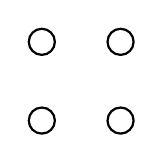
\begin{tikzpicture}[auto,
    specification/.style ={circle, draw, thick}]
   \node[specification] (A) at (0,0)  {};
   \node[specification] (B)  at (0,1)  {};
   \node[specification] (C)  at (1,1)  {};
   \node[specification] (D) at (1,0)  {};
 \end{tikzpicture}\\
 \vspace*{0.3cm}
 A
\end{minipage}\hfill 
  \begin{minipage}{0.24\linewidth}
    \centering
    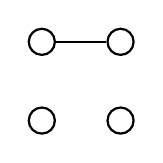
\begin{tikzpicture}[auto,
    specification/.style ={circle, draw, thick}]
   \node[specification] (A) at (0,0)  {};
   \node[specification] (B) at (0,1)  {};
   \node[specification] (C) at (1,1)  {};
   \node[specification] (D) at (1,0)  {};
   \draw[thick] (B) to  (C);
 \end{tikzpicture}\\
 \vspace*{0.3cm}
 B
\end{minipage}\hfill 
  \begin{minipage}{0.24\linewidth}
    \centering
    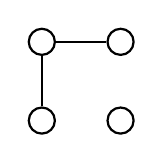
\begin{tikzpicture}[auto,
    specification/.style ={circle, draw, thick}]
   \node[specification] (A) at (0,0)  {};
   \node[specification] (B) at (0,1)  {};
   \node[specification] (C) at (1,1)  {};
   \node[specification] (D) at (1,0)  {};
   \draw[thick] (A) to  (B);
   \draw[thick] (B) to  (C);
 \end{tikzpicture}\\
 \vspace*{0.3cm}
 C
\end{minipage}\hfill 
  \begin{minipage}{0.24\linewidth}
    \centering
    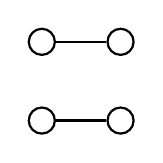
\begin{tikzpicture}[auto,
    specification/.style ={circle, draw, thick}]
   \node[specification] (A)  at (0,0)  {};
   \node[specification] (B)  at (0,1)  {};
   \node[specification] (C)  at (1,1)  {};
   \node[specification] (D) at (1,0)  {};
   \draw[thick] (B) to  (C);
   \draw[thick] (D) to  (A);
 \end{tikzpicture}\\
 \vspace*{0.3cm}
 D
\end{minipage}\hfill

\vspace*{0.5cm}
  \begin{minipage}{0.24\linewidth}
    \centering
    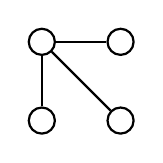
\begin{tikzpicture}[auto,
    specification/.style ={circle, draw, thick}]
   \node[specification] (A) at (0,0)  {};
   \node[specification] (B)  at (0,1)  {};
   \node[specification] (C)  at (1,1)  {};
   \node[specification] (D) at (1,0)  {};
   \draw[thick] (A) to (B);
   \draw[thick] (B) to (C);
      \draw[thick] (B) to (D);
 \end{tikzpicture}\\
 \vspace*{0.3cm}
 E
\end{minipage}\hfill
  \begin{minipage}{0.24\linewidth}
    \centering
    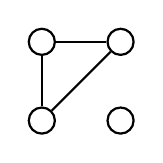
\begin{tikzpicture}[auto,
    specification/.style ={circle, draw, thick}]
   \node[specification] (A) at (0,0)  {};
   \node[specification] (B) at (0,1)  {};
   \node[specification] (C) at (1,1)  {};
   \node[specification] (D) at (1,0)  {};
   \draw[thick] (A) to  (B);
   \draw[thick] (B) to (C);
      \draw[thick] (C) to (A);
 \end{tikzpicture}\\
 \vspace*{0.3cm}
 F
\end{minipage}\hfill
  \begin{minipage}{0.24\linewidth}
    \centering
    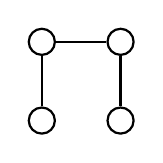
\begin{tikzpicture}[auto,
    specification/.style ={circle, draw, thick}]
   \node[specification] (A) at (0,0)  {};
   \node[specification] (B) at (0,1)  {};
   \node[specification] (C) at (1,1)  {};
   \node[specification] (D) at (1,0)  {};
   \draw[thick] (A) to  (B);
   \draw[thick] (B) to  (C);
      \draw[thick] (C) to (D);
 \end{tikzpicture}\\
 \vspace*{0.3cm}
 G
\end{minipage}\hfill 
  \begin{minipage}{0.24\linewidth}
    \centering
    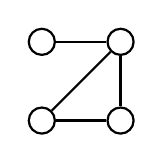
\begin{tikzpicture}[auto,
    specification/.style ={circle, draw, thick}]
   \node[specification] (A)  at (0,0)  {};
   \node[specification] (B)  at (0,1)  {};
   \node[specification] (C)  at (1,1)  {};
   \node[specification] (D) at (1,0)  {};
   \draw[thick] (A) to  (C);
   \draw[thick] (C) to  (D);
   \draw[thick] (D) to (A);
   \draw[thick] (C) to (B);
 \end{tikzpicture}\\
 \vspace*{0.3cm}
 H
\end{minipage}\hfill 

\vspace*{0.5cm}
\flushleft
  \begin{minipage}{0.24\linewidth}
    \centering
    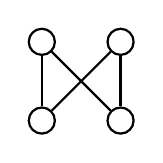
\begin{tikzpicture}[auto,
    specification/.style ={circle, draw, thick}]
   \node[specification] (A) at (0,0)  {};
   \node[specification] (B)  at (0,1)  {};
   \node[specification] (C)  at (1,1)  {};
   \node[specification] (D) at (1,0)  {};
   \draw[thick] (A) to (B);
   \draw[thick] (B) to (D);
   \draw[thick] (D) to (C);
      \draw[thick] (C) to (A);
 \end{tikzpicture}\\
 \vspace*{0.3cm}
 I
\end{minipage}
  \begin{minipage}{0.24\linewidth}
    \centering
    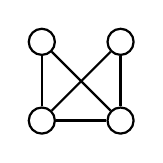
\begin{tikzpicture}[auto,
    specification/.style ={circle, draw, thick}]
   \node[specification] (A) at (0,0)  {};
   \node[specification] (B) at (0,1)  {};
   \node[specification] (C) at (1,1)  {};
   \node[specification] (D) at (1,0)  {};
   \draw[thick] (A) to  (B);
      \draw[thick] (C) to (D);
   \draw[thick] (D) to (A);
   \draw[thick] (A) to (C);
   \draw[thick] (B) to (D);
 \end{tikzpicture}\\
 \vspace*{0.3cm}
 J
\end{minipage} 
  \begin{minipage}{0.24\linewidth}
    \centering
    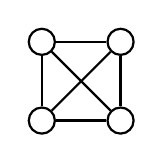
\begin{tikzpicture}[auto,
    specification/.style ={circle, draw, thick}]
   \node[specification] (A) at (0,0)  {};
   \node[specification] (B) at (0,1)  {};
   \node[specification] (C) at (1,1)  {};
   \node[specification] (D) at (1,0)  {};
   \draw[thick] (A) to  (B);
   \draw[thick] (B) to  (C);
      \draw[thick] (C) to (D);
   \draw[thick] (D) to (A);
   \draw[thick] (A) to (C);
   \draw[thick] (B) to (D);
 \end{tikzpicture}\\
 \vspace*{0.3cm}
 K
\end{minipage}

  \begin{Exercise}
    画出具有$3$个顶点的所有有向图(同构的只算一个)。
\end{Exercise}

%  \centering
\begin{minipage}{0.24\linewidth}\centering
  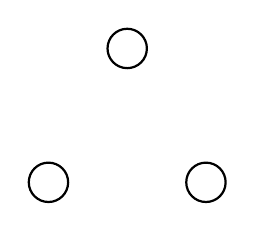
\begin{tikzpicture}[auto,
    specification/.style ={circle, draw, thick,inner sep=0pt, minimum size=5mm}]
   \node[specification] (A)  at (-1,0)  {};
   \node[specification] (B)  at (1,0)  {};
   \node[specification] (C)  at (0,1.7)  {};
 \end{tikzpicture}\\
  \vspace*{0.3cm}
  A
\end{minipage}\hfill
\begin{minipage}{0.24\linewidth}\centering
  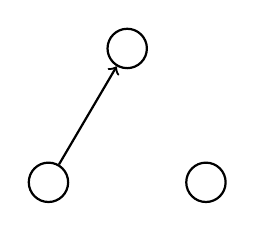
\begin{tikzpicture}[auto,
    specification/.style ={circle, draw, thick,inner sep=0pt, minimum size=5mm}]
   \node[specification] (A)  at (-1,0)  {};
   \node[specification] (B)  at (1,0)  {};
   \node[specification] (C)  at (0,1.7)  {};
   \draw[thick, ->] (A) to  (C);
 \end{tikzpicture}\\
   \vspace*{0.3cm}
B
\end{minipage}\hfill
 \begin{minipage}{0.24\linewidth}\centering
  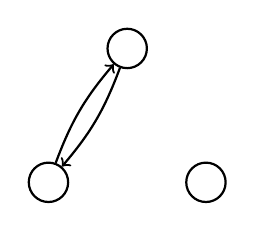
\begin{tikzpicture}[auto,
    specification/.style ={circle, draw, thick,inner sep=0pt, minimum size=5mm}]
   \node[specification] (A)  at (-1,0)  {};
   \node[specification] (B)  at (1,0)  {};
   \node[specification] (C)  at (0,1.7)  {};
   \draw[thick, ->] (A) to  [bend left=10] (C);
   \draw[thick, ->] (C) to  [bend left=10] (A);   
 \end{tikzpicture}\\
   \vspace*{0.3cm}
C
\end{minipage}\hfill
 \begin{minipage}{0.24\linewidth}\centering
  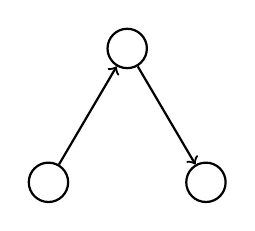
\begin{tikzpicture}[auto,
    specification/.style ={circle, draw, thick,inner sep=0pt, minimum size=5mm}]
   \node[specification] (A)  at (-1,0)  {};
   \node[specification] (B)  at (1,0)  {};
   \node[specification] (C)  at (0,1.7)  {};
   \draw[thick, ->] (A) to  (C);
   \draw[thick, ->] (C) to  (B);
 \end{tikzpicture}\\
   \vspace*{0.3cm}
D
\end{minipage}

\vspace{0.3cm}
 \begin{minipage}{0.24\linewidth}\centering
  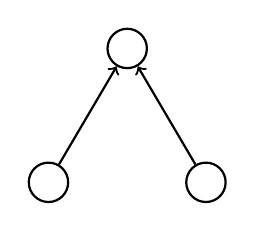
\begin{tikzpicture}[auto,
    specification/.style ={circle, draw, thick,inner sep=0pt, minimum size=5mm}]
   \node[specification] (A)  at (-1,0)  {};
   \node[specification] (B)  at (1,0)  {};
   \node[specification] (C)  at (0,1.7)  {};
   \draw[thick, ->] (A) to  (C);
   \draw[thick, ->] (B) to  (C);
\end{tikzpicture}\\
  \vspace*{0.3cm}
  E
\end{minipage}\hfill
 \begin{minipage}{0.24\linewidth}\centering
  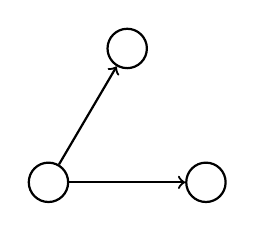
\begin{tikzpicture}[auto,
    specification/.style ={circle, draw, thick,inner sep=0pt, minimum size=5mm}]
   \node[specification] (A)  at (-1,0)  {};
   \node[specification] (B)  at (1,0)  {};
   \node[specification] (C)  at (0,1.7)  {};
   \draw[thick, ->] (A) to  (C);
   \draw[thick, ->] (A) to  (B);
\end{tikzpicture}\\
  \vspace*{0.3cm}
  F
\end{minipage}\hfill
 \begin{minipage}{0.24\linewidth}\centering
  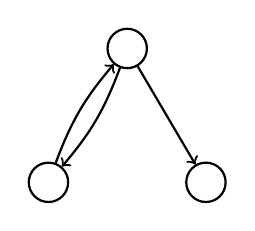
\begin{tikzpicture}[auto,
    specification/.style ={circle, draw, thick,inner sep=0pt, minimum size=5mm}]
   \node[specification] (A)  at (-1,0)  {};
   \node[specification] (B)  at (1,0)  {};
   \node[specification] (C)  at (0,1.7)  {};
   \draw[thick, ->] (A) to  [bend left=10] (C);
   \draw[thick, ->] (C) to  [bend left=10] (A);
   \draw[thick, ->] (C) to  (B);   
\end{tikzpicture}\\
  \vspace*{0.3cm}
  G
\end{minipage}\hfill
 \begin{minipage}{0.24\linewidth}\centering
  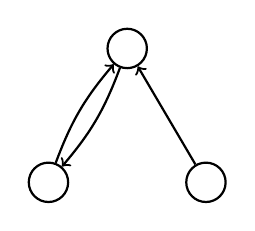
\begin{tikzpicture}[auto,
    specification/.style ={circle, draw, thick,inner sep=0pt, minimum size=5mm}]
   \node[specification] (A)  at (-1,0)  {};
   \node[specification] (B)  at (1,0)  {};
   \node[specification] (C)  at (0,1.7)  {};
   \draw[thick, ->] (A) to  [bend left=10] (C);
   \draw[thick, ->] (C) to  [bend left=10] (A);
   \draw[thick, ->] (B) to  (C);
 \end{tikzpicture}\\
  \vspace*{0.3cm}
  H
\end{minipage}

\vspace{0.3cm}
 \begin{minipage}{0.24\linewidth}\centering
  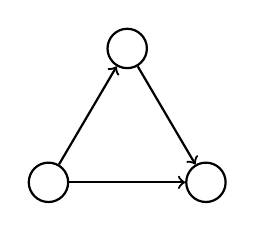
\begin{tikzpicture}[auto,
    specification/.style ={circle, draw, thick,inner sep=0pt, minimum size=5mm}]
   \node[specification] (A)  at (-1,0)  {};
   \node[specification] (B)  at (1,0)  {};
   \node[specification] (C)  at (0,1.7)  {};
   \draw[thick, ->] (A) to  (C);
   \draw[thick, ->] (C) to  (B);
   \draw[thick, ->] (A) to  (B);   
\end{tikzpicture}\\
  \vspace*{0.3cm}
  I
\end{minipage}\hfill
 \begin{minipage}{0.24\linewidth}\centering
  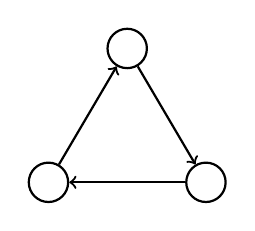
\begin{tikzpicture}[auto,
    specification/.style ={circle, draw, thick,inner sep=0pt, minimum size=5mm}]
   \node[specification] (A)  at (-1,0)  {};
   \node[specification] (B)  at (1,0)  {};
   \node[specification] (C)  at (0,1.7)  {};
   \draw[thick, ->] (A) to  (C);
   \draw[thick, ->] (C) to  (B);
   \draw[thick, ->] (B) to  (A);
 \end{tikzpicture}\\
  \vspace*{0.3cm}
  J
\end{minipage}\hfill
 \begin{minipage}{0.24\linewidth}\centering
  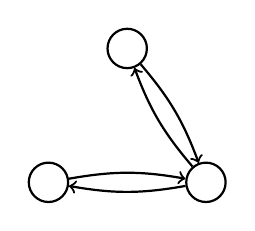
\begin{tikzpicture}[auto,
    specification/.style ={circle, draw, thick,inner sep=0pt, minimum size=5mm}]
   \node[specification] (A)  at (-1,0)  {};
   \node[specification] (B)  at (1,0)  {};
   \node[specification] (C)  at (0,1.7)  {};
   \draw[thick, ->] (A) to  [bend left=10] (B);
   \draw[thick, ->] (B) to  [bend left=10] (A);
   \draw[thick, ->] (B) to  [bend left=10] (C);
   \draw[thick, ->] (C) to  [bend left=10] (B);
 \end{tikzpicture}\\
  \vspace*{0.3cm}
  K
\end{minipage}\hfill
 \begin{minipage}{0.24\linewidth}\centering
  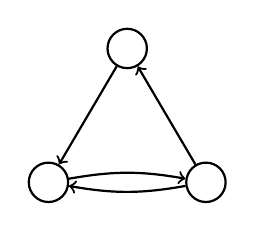
\begin{tikzpicture}[auto,
    specification/.style ={circle, draw, thick,inner sep=0pt, minimum size=5mm}]
   \node[specification] (A)  at (-1,0)  {};
   \node[specification] (B)  at (1,0)  {};
   \node[specification] (C)  at (0,1.7)  {};
   \draw[thick, ->] (A) to  [bend left=10] (B);
   \draw[thick, ->] (B) to  [bend left=10] (A);
   \draw[thick, ->] (B) to  (C);
   \draw[thick, ->] (C) to  (A);
 \end{tikzpicture}\\
  \vspace*{0.3cm}
  L
\end{minipage}

\vspace{0.3cm}
 \begin{minipage}{0.24\linewidth}\centering
   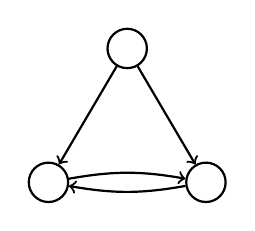
\begin{tikzpicture}[auto,
    specification/.style ={circle, draw, thick,inner sep=0pt, minimum size=5mm}]
   \node[specification] (A)  at (-1,0)  {};
   \node[specification] (B)  at (1,0)  {};
   \node[specification] (C)  at (0,1.7)  {};
   \draw[thick, ->] (A) to  [bend left=10] (B);
   \draw[thick, ->] (B) to  [bend left=10] (A);
   \draw[thick, ->] (C) to  (B);
   \draw[thick, ->] (C) to  (A);
 \end{tikzpicture}\\
  \vspace*{0.3cm}
  M
\end{minipage}\hfill
 \begin{minipage}{0.24\linewidth}\centering
  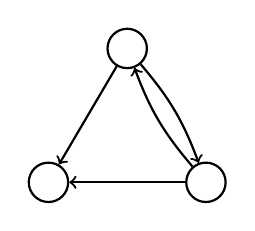
\begin{tikzpicture}[auto,
    specification/.style ={circle, draw, thick,inner sep=0pt, minimum size=5mm}]
   \node[specification] (A)  at (-1,0)  {};
   \node[specification] (B)  at (1,0)  {};
   \node[specification] (C)  at (0,1.7)  {};
   \draw[thick, ->] (C) to   (A);
   \draw[thick, ->] (B) to   (A);
   \draw[thick, ->] (B) to  [bend left=10] (C);
   \draw[thick, ->] (C) to  [bend left=10] (B);
 \end{tikzpicture}\\
  \vspace*{0.3cm}
  N
\end{minipage}\hfill
 \begin{minipage}{0.24\linewidth}\centering
  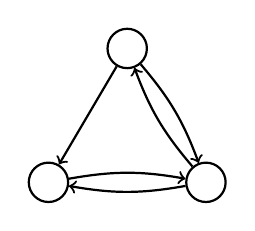
\begin{tikzpicture}[auto,
    specification/.style ={circle, draw, thick,inner sep=0pt, minimum size=5mm}]
   \node[specification] (A)  at (-1,0)  {};
   \node[specification] (B)  at (1,0)  {};
   \node[specification] (C)  at (0,1.7)  {};
   \draw[thick, ->] (A) to  [bend left=10] (B);
   \draw[thick, ->] (B) to  [bend left=10] (A);
   \draw[thick, ->] (B) to  [bend left=10] (C);
   \draw[thick, ->] (C) to  [bend left=10] (B);
   \draw[thick, ->] (C) to   (A);   
 \end{tikzpicture}\\
  \vspace*{0.3cm}
  O
\end{minipage}\hfill
 \begin{minipage}{0.24\linewidth}\centering
  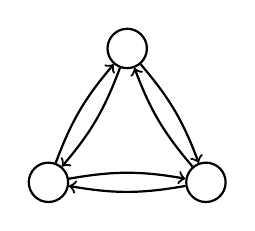
\begin{tikzpicture}[auto,
    specification/.style ={circle, draw, thick,inner sep=0pt, minimum size=5mm}]
   \node[specification] (A)  at (-1,0)  {};
   \node[specification] (B)  at (1,0)  {};
   \node[specification] (C)  at (0,1.7)  {};
   \draw[thick, ->] (A) to  [bend left=10] (B);
   \draw[thick, ->] (B) to  [bend left=10] (A);
   \draw[thick, ->] (B) to  [bend left=10] (C);
   \draw[thick, ->] (C) to  [bend left=10] (B);
   \draw[thick, ->] (A) to  [bend left=10] (C);
   \draw[thick, ->] (C) to  [bend left=10] (A);   
 \end{tikzpicture}\\
  \vspace*{0.3cm}
  P
\end{minipage}

  \begin{Exercise}
  画出具有4个,6个,8个顶点的三次图。
\end{Exercise}
%  \begin{proof}[解]
    \begin{minipage}{0.3\linewidth}
    \centering
    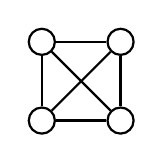
\begin{tikzpicture}[auto,
    specification/.style ={circle, draw, thick}]
   \node[specification] (A) at (0,0)  {};
   \node[specification] (B) at (0,1)  {};
   \node[specification] (C) at (1,1)  {};
   \node[specification] (D) at (1,0)  {};
   \draw[thick] (A) to  (B);
   \draw[thick] (B) to  (C);
   \draw[thick] (C) to (D);
   \draw[thick] (D) to (A);
   \draw[thick] (A) to (C);
   \draw[thick] (B) to (D);
 \end{tikzpicture}
\end{minipage}
    \begin{minipage}{0.3\linewidth}
    \centering
    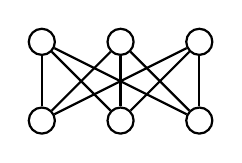
\begin{tikzpicture}[auto,
    specification/.style ={circle, draw, thick}]
   \node[specification] (A) at (0,0)  {};
   \node[specification] (B) at (1,0)  {};
   \node[specification] (C) at (2,0)  {};
   \node[specification] (D) at (0,1)  {};
   \node[specification] (E) at (1,1)  {};
   \node[specification] (F) at (2,1)  {};
   \draw[thick] (A) to  (D);
   \draw[thick] (A) to  (E);
   \draw[thick] (A) to (F);
   \draw[thick] (B) to (D);
   \draw[thick] (B) to (E);
   \draw[thick] (B) to (F);
   \draw[thick] (C) to (D);
   \draw[thick] (C) to (E);
   \draw[thick] (C) to (F);
 \end{tikzpicture}
\end{minipage}
    \begin{minipage}{0.3\linewidth}
    \centering
    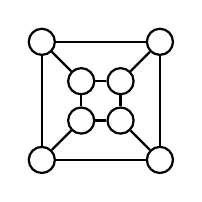
\begin{tikzpicture}[auto,
    specification/.style ={circle, draw, thick}]
   \node[specification] (A) at (0,0)  {};
   \node[specification] (B) at (1/2,1/2)  {};
   \node[specification] (C) at (1,1/2)  {};
   \node[specification] (D) at (3/2,0)  {};
   \node[specification] (E) at (0,3/2)  {};
   \node[specification] (F) at (1/2,1)  {};
   \node[specification] (G) at (1,1)  {};
   \node[specification] (H) at (3/2,3/2)  {};
   
   \draw[thick] (A) to  (B);
   \draw[thick] (B) to  (C);
   \draw[thick] (C) to (D);
   \draw[thick] (D) to (A);
   \draw[thick] (E) to  (F);
   \draw[thick] (F) to  (G);
   \draw[thick] (G) to (H);
   \draw[thick] (H) to (E);
   \draw[thick] (A) to  (E);
   \draw[thick] (B) to  (F);
   \draw[thick] (C) to (G);
   \draw[thick] (D) to (H);
 \end{tikzpicture}
\end{minipage}

\end{proof}
  \input{p206-4-exercise}
%  \input{p206-4-answer}
  \input{p209-1-exercise}
%  \begin{proof}[答]
  设$u$与$v$是图$G$的两个不同顶点。如果$u$与$v$间有两条不同的通道,则$G$中不一定有圈。举例如下:考虑$G=(\{u,v\},\{(u,v)\})$,则$uv$和$uvuv$为$u$与$v$间两条不同的通道,但$G$中没有圈。

  如果$u$与$v$间有两条不同的迹,则$G$中一定有圈。证明如下:设$u$与$v$间有两条不同的迹$T_1$和$T_2$。如果$T_1$和$T_2$都为路,则$G$中有圈;如果$T_1=uv_1v_2\ldots v_nv$不是路,设$v_j=v_i(i<j)$为第一个重复的顶点,则$v_iv_{i+1}\ldots v_j$构成$G$中的一个圈;同理,如果$T_2$不是路,$G$中有圈。
  
\end{proof}
  \begin{Exercise}
    证明:一个连通的$(p,q)$图中$q\geq p - 1$。  
\end{Exercise}

%  \input{p209_2_answer}
  \begin{Exercise}
    若$G$是一个$(p,q)$图,$q > \frac{1}{2}(p-1)(p-2)$,试证$G$是连通图。  
\end{Exercise}

%  \begin{proof}[证明]
      用反证法。假设$G$不连通,则至少有两个连通分量。设其中一个连通分量的顶点数为
    $p_1$,边数为$q_1$,所有其他连通分量的顶点数为$p_2$,边数为$q_2$。则
    \begin{equation*}
      \begin{split}
        &\frac{1}{2}(p-1)(p-2)\\
        =&\frac{1}{2}(p_1 + p_2 -1)(p_1 + p_2 -2)\\
        =&\frac{1}{2}(p_1 + p_2 -1)((p_1 - 1) + (p_2 - 1))\\
        =&\frac{1}{2}(p_1(p_1 -1) +  p_1(p_2 - 1) + p_2(p_1 - 1) + p_2(p_2-1) - (p_1 - 1) - (p_2-1))\\
        =&\frac{1}{2}(p_1(p_1 -1) +   p_2(p_2-1) + 2(p_1 - 1)(p_2-1))\\
        =&\frac{p_1(p_1 -1)}{2} +   \frac{p_2(p_2-1)}{2} + (p_1 - 1)(p_2-1))\\
        \geq&\frac{p_1(p_1 -1)}{2} +   \frac{p_2(p_2-1)}{2}\\
        \geq & q
      \end{split}
    \end{equation*}
    矛盾。
\end{proof}

%  \input{p209_6_exerise}
%  \input{p209_6_answer}
  \begin{Exercise}
    设$G$为图。证明:若$\delta(G)\geq 2$,则$G$包含长度至少为$\delta(G)+1$的圈。  
\end{Exercise}

%  \begin{proof}[证明]
      设$P=v_0v_1\ldots v_n$为$G$中的一条最长路,则$v_0$只能与$P$中的顶点相邻接,否则假设$v_0$与不在$P$中的顶点$u$邻接,则$uv_0v_1\ldots v_n$构成了$G$中一条更长的路,与$P$为$G$中的最长路矛盾。取最大的$s$使得$v_0$与$v_s$相邻接,则$C=v_0v_1\ldots v_sv_0$为长度至少为$\delta(G)+1$的圈,这是因为$v_0$至少与$\delta(G)$个顶点相邻接,而所有这些与$v_0$邻接的顶点均在圈$C$中。
\end{proof}

  \begin{Exercise}
  证明:如果图$G$不是连通图,则$G^c$是连通图。
\end{Exercise}

%  \begin{proof}[证明]
  设$u$和$v$为$G^c$中的任意两个不同的顶点。如果$u$和$v$不在$G$的同一个连通分量中,则$uv$不是$G$的一条边,于是$uv$为$G^c$的一条边,从而在$G^c$中$u$和$v$之间存在一条路;如果$u$和$v$在$G$的同一个连通分量中,取$G$的另外一个连通分量中的一个顶点$w$,则$uw$和$wv$都不是$G$中的边,从而为$G^c$中的边,于是$uwv$构成了$G^c$中$u$和$v$之间的一条路。
\end{proof}

  \begin{Exercise}
 证明:每一个自补图有$4n$或$4n+1$个顶点。
\end{Exercise}

%  \begin{proof}[证明]
  设$G$为自补图,有$p$个顶点,则$G$和$G^c$共有$p(p-1)/2$条边。由$G$为自补图知,$G$和$G^c$有相同的边数,从而$p(p-1)/2$能被$2$整除。只有当$p=4n$或$p=4n+1$时,$p(p-1)/2$能被$2$整除,结论得证。
\end{proof}

  \begin{Exercise}
  给出一个$10$个顶点的非哈密顿图的例子,使得每一对不邻接的顶点$u$和$v$,均有$\deg u + \deg v \geq 9$。
\end{Exercise}

%  \begin{proof}[解]
  $K_9$外再连接一个顶点。
\end{proof}

  \begin{Exercise}
  试求$K_p$中不同的哈密顿圈的个数。
\end{Exercise}

%  \begin{proof}[解]
  $\frac{(p-1)!}{2}$
\end{proof}

  \begin{Exercise}
  完全偶图$K_{m,n}$为哈密顿图的充分必要条件是什么?
\end{Exercise}

%  \begin{proof}[解]
  $m=n$。
\end{proof}

  \begin{Exercise}
  证明具有奇数个顶点的偶图不是哈密顿图。
\end{Exercise}

%  \begin{proof}[证明]
  设$G$为偶图,其顶点即可以划分为两个集合$V_1$和$V_2$,使得任意一条边一个顶点在$V_1$中,一个顶点在$V_2$中。如果$G$有奇数个顶点,则$|V_1|\neq |V_2|$。不妨设$|V_1| < |V_2|$,则$\omega (G-V_1) > |V_1|$,从而$G$不是哈密顿图。
\end{proof}


\end{CJK}
\end{document}


%%% Local Variables:
%%% mode: latex
%%% TeX-master: t
%%% End:
